

\tikzset{every picture/.style={line width=0.75pt}} %set default line width to 0.75pt        

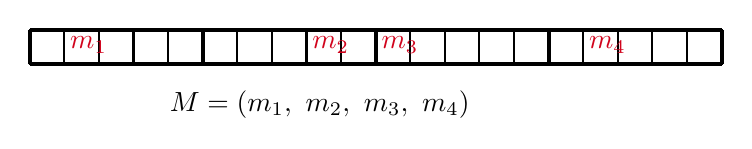
\begin{tikzpicture}[x=0.5pt,y=0.5pt,yscale=-1,xscale=1]
%uncomment if require: \path (0,88); %set diagram left start at 0, and has height of 88

%Shape: Grid [id:dp7159974501706334] 
\draw  [draw opacity=0][line width=0.75]  (15,13) -- (515,13) -- (515,38) -- (15,38) -- cycle ; \draw  [line width=0.75]  (40,13) -- (40,38)(65,13) -- (65,38)(90,13) -- (90,38)(115,13) -- (115,38)(140,13) -- (140,38)(165,13) -- (165,38)(190,13) -- (190,38)(215,13) -- (215,38)(240,13) -- (240,38)(265,13) -- (265,38)(290,13) -- (290,38)(315,13) -- (315,38)(340,13) -- (340,38)(365,13) -- (365,38)(390,13) -- (390,38)(415,13) -- (415,38)(440,13) -- (440,38)(465,13) -- (465,38)(490,13) -- (490,38) ; \draw  [line width=0.75]   ; \draw  [line width=0.75]  (15,13) -- (515,13) -- (515,38) -- (15,38) -- cycle ;
%Straight Lines [id:da4276676225384277] 
\draw [line width=1.5]    (15,38) -- (515,38) ;
%Straight Lines [id:da38414129135222486] 
\draw [line width=1.5]    (15,13) -- (515,13) ;
%Straight Lines [id:da8193193450080452] 
\draw [line width=1.5]    (15,38) -- (15,13) ;
%Straight Lines [id:da4559031610077283] 
\draw [line width=1.5]    (140,38) -- (140,13) ;
%Straight Lines [id:da7340056619830325] 
\draw [line width=1.5]    (515,38) -- (515,13) ;
%Straight Lines [id:da6116177459817139] 
\draw [line width=1.5]    (265,38) -- (265,13) ;
%Straight Lines [id:da4924257748666654] 
\draw [line width=1.5]    (390,38) -- (390,13) ;

% Text Node
\draw (42,16) node [anchor=north west][inner sep=0.75pt]   [align=left] {$\displaystyle \textcolor[rgb]{0.82,0.01,0.11}{m_{1}}$};
% Text Node
\draw (217,16) node [anchor=north west][inner sep=0.75pt]   [align=left] {$\displaystyle \textcolor[rgb]{0.82,0.01,0.11}{m}\textcolor[rgb]{0.82,0.01,0.11}{_{2}}$};
% Text Node
\draw (267,16) node [anchor=north west][inner sep=0.75pt]   [align=left] {$\displaystyle \textcolor[rgb]{0.82,0.01,0.11}{m}\textcolor[rgb]{0.82,0.01,0.11}{_{3}}$};
% Text Node
\draw (417,16) node [anchor=north west][inner sep=0.75pt]   [align=left] {$\displaystyle \textcolor[rgb]{0.82,0.01,0.11}{m}\textcolor[rgb]{0.82,0.01,0.11}{_{4}}$};
% Text Node
\draw (114,55) node [anchor=north west][inner sep=0.75pt]   [align=left] {$\displaystyle M=( m_{1} ,\ m_{2} ,\ m_{3} ,\ m_{4})$};


\end{tikzpicture}
